\documentclass[preprint,amsmath,amssymb,superscriptaddress]{revtex4-1}
%\documentclass[twocolumn,amsmath,amssymb,superscriptaddress]{revtex4-1}
\usepackage{graphicx,amsmath}
\usepackage{xcolor}
\usepackage{xr}
\externaldocument[S-]{Supplementary}
\begin{document}
%\draft


\title{Formation of porous crystals via viscoelastic phase separation} 

\author{Hideyo Tsurusawa} 
\affiliation{Institute of Industrial Science, University of Tokyo, 4-6-1 Komaba, Meguro-ku, Tokyo 153-8505, Japan}
\author{John Russo}
\affiliation{Institute of Industrial Science, University of Tokyo, 4-6-1 Komaba, Meguro-ku, Tokyo 153-8505, Japan}
\affiliation{ {School of Mathematics, University of Bristol, Bristol BS8 1TW, United Kingdom} }
\author{Mathieu Leocmach}
\affiliation{Institut Lumière Matière, CNRS UMR 5306, Université Claude Bernard Lyon 1, Université de Lyon, Lyon, 69622 Villeurbanne Cedex, France}
\author{Hajime Tanaka  \footnote{e-mail: tanaka@iis.u-tokyo.ac.jp}}
\affiliation{Institute of Industrial Science, University of Tokyo, 4-6-1 Komaba, Meguro-ku, Tokyo 153-8505, Japan}

\date{Received July 20, 2016}

\begin{abstract}
{\bf
Viscoelastic phase separation of colloidal suspensions can be interrupted to form gels either by 
%the glass transition, with the formation of colloidal gels~\cite{poon2002,zaccarelli2007,piazza1994phase,verhaegh1997transient,tanaka1999colloid,lu2008gelation}, or by crystallization, which results in the formation of a crystalline network~\cite{soga1999metastable,fortini2008crystallization,perez2011pathways,sabin2012}. 
glass transition
%~\cite{poon2002,zaccarelli2007,piazza1994phase,verhaegh1997transient,tanaka1999colloid,lu2008gelation} 
or by crystallization. 
%~\cite{soga1999metastable,fortini2008crystallization,perez2011pathways,sabin2012,zhang2012non}. 
%But while the former process has been studied in detail, the latter has never been observed experimentally at a single-particle level and it is thus lacking a microscopic understanding. 
With a new confocal microscopy protocol, \textcolor{blue}{we follow the entire kinetics of phase separation, from the homogeneous phase to the formation of different arrested states.
This allows us to unveil a novel crystallization pathway to sponge-like porous crystal structures in a colloid-polymer mixture undergoing viscoelastic gas-liquid phase separation.
We show that crystallization is preceeded by a structural reorganization of the liquid phase, called stress-driven aging.
Nucleation starts inside this liquid network, but crystals grow past it by direct condensation of the gas phase on their surface, i.e. de-sublimation, driving evaporation of nearby liquid. This produces a network structure different from the original phase separation pattern.}
%The latter processes via the gas phase has been overlooked so far. %This process represents the colloidal analogue of the Bergeron process~\cite{glickman2000glossary}, which explains the formation of ice crystals in mixed phase clouds and is at the origin of rain. Our finding gives us full experimental access to the kinetic pathway of this poorly understood phenomenon important for climate science. 
%The key is complex dynamic interplay involving the three phases upon simultaneous occurrence of two non-equilibrium phenomena, phase separation and crystallization. 
We argue that similar crystal-gel states can be formed as the result of the gas-liquid phase separation of any crystallizable components, such as monoatomic and molecular systems, if dynamics of the liquid phase is slow enough to induce viscoelastic phase separation, but fast enough to prevent immediate vitrification. This mechanism will provide a novel pathway to form nano-porous crystals of metals and semiconductors without dealloying, %\cite{erlebacher2001evolution}, 
which may be important for catalytic, optical, sensing, and filtration applications. 
%\cite{ding2004nanoporous,ding2009nanoporous, wittstock2010nanoporous}.
%, but also sheds new light on crystal network formation in more complex systems such as magma \cite{philpotts1998role}, biominerals \cite{rousseau2005multiscale}, and foods \cite{deman1987fat}.}
}
\end{abstract}


\maketitle

%\subsection{Introduction}

Crystallization plays a fundamental role in many processes occurring in nature, such as \textcolor{blue}{ice formation in atmospheric clouds \cite{glickman2000glossary,morrison2012resilience}}, and in technological applications
that are at the core of the chemical, pharmaceutical, and food industries.
Many of the properties of crystals, like the shape, spatial arrangement, polymorph type, and size distribution of the crystallites, depend on the conditions at which
the nucleation process took place. Controlling the early stages of crystallization is thus of fundamental importance in order to
obtain in a reproducible manner crystals with the desired properties. 

%\textcolor{brown}{Mathieu: When I presented this story, I was often told that our initial focus on nucleation was misleading since our main result is about growth. What about trimming down this part? Or focussing more on growth rather than nucleation?}
Under usual conditions, the nucleation stage involves a very small number of molecules, of the order of 10-1000 molecules.
This has severely limited the possibility to observe the  \textcolor{blue}{crystallization} process directly, and has also posed limits on models based on macroscopic thermodynamic properties. 
The inability to directly observe the  \textcolor{blue}{crystallization} process is also a limit to our understanding of its kinetic pathway. 
Classical Nucleation Theory assumes the crystallization processes to occur in one step,
where the transition can be described by just one reaction coordinate. An example is the formation of an ordered crystalline nucleus
directly from the supersaturated solution. But the possibility of different pathways has recently come to prominence with
the discovery of two-step nucleation pathways, where crystallization is proceeded by the formation of dense liquid  droplets as an intermediate step~\cite{ten1997enhancement,SearR,savage2009experimental,vekilov2010two,palberg2014crystallization}.
Understanding the process of crystal formation in mixed-phase systems (composed of gas, liquid, and solid phases) is thus
of great importance for a variety of systems, from protein solutions to clouds. 

Colloidal suspensions offer a system where the crystallization process in a mixed-phase environment can be observed with single-particle
resolution, and at the same time scales over which nucleation takes place. In colloids with short-range attractions the liquid-gas transition 
becomes metastable with respect to crystallization~\cite{anderson2002insights,lekkerkerker2011colloids}, and can form gels.  
~\cite{poon2002,zaccarelli2007,piazza1994phase,verhaegh1997transient,lu2008gelation}. 
\textcolor{blue}{This gel formation process can be regarded as viscoelastic phase separation  \cite{tanaka1999colloid,tanaka2000viscoelastic} into a dense liquid phase with slow dynamics and a dilute gas phase with fast dynamics.} 
This difference in the viscoelastic properties between the two phases allows the system to form a space-spanning 
network structure of the liquid phase, even if it is the minority phase. The network is fractal and its dynamic structure factor shows a stretched-exponential decay to a finite
plateau~\cite{krall1998internal,solomon2001dynamic,romer2000sol}. 
During phase separation, the density of the liquid phase increases towards the glass-transition density, leading to slow glassy dynamics.
At the glass transition point, the percolated network structure is dynamically stabilised by vitrification 
of the dense liquid phase~\cite{pusey1993dynamics,piazza1994phase,ilett1995phase,verhaegh1997transient,tanaka1999colloid,foffi2002,buzzaccaro2007sticky,zaccarelli2007,lu2008gelation,zaccarelli2008gelation,testard2011}.  
More precisely, the dynamical stabilization is due to percolation of locally favoured structures, which are locally stable non-crystalline structures \cite{royall2008g}.

% Gels and glasses are two important non-ergodic disordered states, which are very important 
% in our life and nature~\cite{anderson2002insights,lekkerkerker2011colloids}.
% The dynamical arrest of colloidal gels and glasses is believed to originate from a dynamical transition to the same non-ergodic disordered glass state, i.e., vitrification. The only difference comes from the fact that the former is formed by densification induced by phase separation and thus is spatially heterogeneous, whereas the latter is formed by uniform densification and is thus spatially homogeneous.
% Gels are distinct from glasses because of their heterogeneous network structure, which gives them properties intermediate between
% those of a solid and a fluid phase, and allows the coexistence of two properties usually incompatible with each other, 
% elasticity and fluidity. 
% The elasticity of gels originates from the percolated network structure and the resulting space-spanning connectivity. 
% At the same time a fluid component can easily flow through the elastic network.
% There are two types of gels with such characteristics: one is a network structure stabilized by stable crosslinks, and the other is a phase-separated structure frozen by dynamical arrest due to vitrification.
% Many chemical and physical gels belong to the former category, in which the size of network pores is rather small and 
% the fluid transport is not so efficient. On the other hand, gels made of spherical colloids and proteins 
% with attractive interactions belong to the latter category. 
% This type of gels are formed by viscoelastic phase separation \cite{tanaka1999colloid,tanaka2000viscoelastic} into a dense liquid phase with slow dynamics and a dilute gas phase 
% with fast dynamics. This difference in the viscoelastic properties between the two phases allows the system to form a space-spanning 
% network structure of the liquid phase, even if it is the minority phase. The network is fractal and its dynamic structure factor shows a stretched-exponential decay to a finite
% plateau~\cite{krall1998internal,solomon2001dynamic,romer2000sol}. During phase separation, the density of the liquid phase 
% increases towards the glass-transition density, leading to slow glassy dynamics.
% At the glass transition point, the percolated network structure is dynamically stabilised by vitrification 
% of the dense liquid phase~\cite{pusey1993dynamics,ilett1995phase,verhaegh1997transient,tanaka1999colloid,foffi2002,buzzaccaro2007sticky,zaccarelli2007,lu2008gelation,zaccarelli2008gelation,testard2011}.  
% More precisely, the dynamical stabilization is due to percolation of locally favored structures, which are locally stable non-crystalline structures \cite{royall2008g}.
% Since ``glass'' is the term used for bulk, this may be a more appropriate way to express the mechanism of dynamical arrest. 
% This type of gels are made by phase separation. Thus, the structure is intrinsically heterogeneous, and the network pore size is usually 
% much larger than gels made of stable crosslinks, resulting in a high fluid transport ability. 

\textcolor{blue}{Unlike the above standard scenario of colloidal gelation, it is known that phase separation can also be accomapnied by crystallization \cite{poon1999cpm,renth2001phase}, if the process takes place below the melting point of one of the two separating phases}~\cite{tanaka1985new}. Indeed the possibility of a different class of gels, which are stabilized by crystallization, 
was suggested by numerical simulations~\cite{soga1999metastable,fortini2008crystallization,perez2011pathways} and observed in experiments \cite{sabin2012,zhang2012non}. \textcolor{blue}{Such crystallization upon gel formation was also observed 
for a system of oppositely charged colloids \cite{sanz2008gel,sanz2008out}.}  
For colloidal systems, we can in principle access structural evolution in real time at a single-particle level; however, there has so far been no confocal microscopy  
studies on the dynamical process of crystal-gel formation on a microscopic level, which makes the microscopic mechanism of crystal-gel formation elusive. 
For confocal microscopy experiments on colloid gelation, colloid-polymer mixtures have so far been used as a model system. 
The main difficulty consists in the preparation protocol of such a colloid-polymer mixture where, before observation of its dynamics, shaking or applying shear is necessary to prepare an initial homogeneous state. This introduces turbulent flows at the beginning of the process, and also does not allow the
observation of the initial stages of  \textcolor{blue}{gelation}. This initial perturbation may even alter the selection of the final non-equilibrium arrested state.  
In our experiments we instead succeed in building a novel protocol that allows the time evolution of the system to be observed directly
under the confocal microscope from the very early stages and in a quiescent situation without introducing fluid flows. 

\textcolor{blue}{
In this Letter, we show that the system can undergo a novel crystallization pathway that leads to the formation of interconnected crystalline droplets. 
These droplets originate from crystal seeds that form inside the liquid branches of the spinodal aggregate of network morphology.
We show that a necessary condition for the nucleation of crystal seeds is the stress-driven aging of the network which releases the stresses that build-up during the network formation due to hydrodynamic interactions, allowing for an increase in the number of average neighbours. 
If the average concentration of particles is high enough, this stress relaxation triggers the nucleation process of crystals. 
Stress-driven ageing is possible only at low polymer concentration. 
Indeed, at higher polymer concentration (i.e., under stronger interparticle attraction) we observe that, instead of forming crystal gels, the system undergoes the classical gelation process, in which
phase separation is interrupted by vitrification~\cite{verhaegh1997transient,tanaka1999colloid,Royall2007,lu2008gelation}.
We then show that the growth of the crystal seeds occurs by three different routes:
(i) growth within the dense branches of the gel;
(ii) Bergeron process, analogous to ice formation in mixed phase clouds \cite{glickman2000glossary,morrison2012resilience}, where ice droplets grow at the
expense of the supercooled liquid droplets due to their lower saturated vapour pressure;
(iii) Ostwald ripening.
Differently from the standard crystal-gel scenario, where crystals only nucleate and grow inside the dense branches of the gel, becoming dynamically arrested, we show that the kinetic pathways involving the gas phase (predominantly the Bergeron process, but also Ostwald ripening) play an important role.
We reveal that the final crystal-gel network structure has smoother interface than the ordinary gels formed by vitrification because of this novel crystal growth mechanism.
}

%\subsection{Samples}
\begin{figure}[h]
 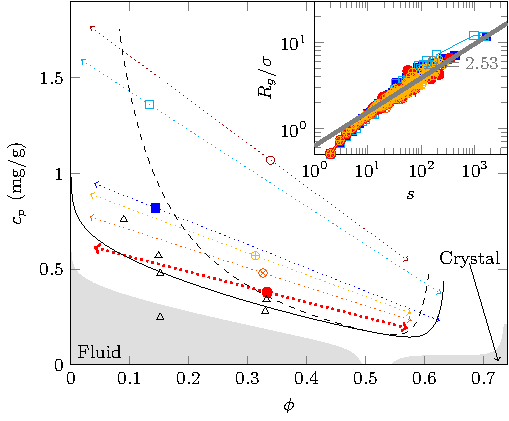
\includegraphics[width=8cm]{network_formation.pdf}
 \caption{\textcolor{blue}{{\bf Phase behaviour.}} 
Empty black triangles are experimental points showing fluid behaviour. The other symbols are the experimental points showing gel behaviour, consistently used in all figures. The dotted lines are the gas-liquid tie lines determined experimentally, with arrow heads indicating measured gas and liquid compositions (see Supplementary Information on the procedure to extract the compositions from confocal images).  Gray areas are theoretical equilibrium fluid and crystal regions. The solid and dashed lines are the metastable gas-liquid binodal and spinodal respectively.
\textbf{(Inset)} Radius of gyration ($R_g$) as a function of cluster size ($s$) for all state points at percolation time. The gray line represents the fractal dimension of the random gelation universality class \textcolor{blue}{($D=2.53$)}.
 }
 \label{fig:network_formation}
\end{figure}


In our experimental setup, the sample cell is put in contact with a reservoir of a salt solution through a semi-permeable membrane (see Methods 
on the details of our experiments).
At $t=0$, the increase in the concentration of salt ions within a few Brownian times ($\tau_{\rm B}$) screens the Coulomb repulsion between colloidal particles,
which are then subject to attractive depletion forces, making the system thermodynamically unstable and leading to phase separation. 
%In the following we discuss all the stages of the formation of the crystal gels: phase separation, stress-driven agein and crystallization.
The experimental data are taken at two different volume fractions ($\phi\approx 0.14$ and $\phi\approx 0.33$) and for different values
of the polymer concentration, $c_p=0.38,0.48,0.57,1.07$ mg/g for $\phi\approx 0.33$ and $c_p=0.82,1.36$ mg/g for $\phi\approx 0.14$.
In Fig.~\ref{fig:network_formation}, we superimpose the state points with a theoretical phase diagram, which we calculated from generalised free volume theory~\cite{Fleer2008} using the experimental values for the size of the colloids, the radius of gyration of the polymer, and the polymer concentration (see Supplementary Methods).
For each state point, scans were made at early times (every $10$~s, i.e. $4\tau_{\rm B}$) and at the late stage (every $30$~s) of the gelation process. 


%
%\subsection*{Phase separation}
%
%In Fig.~\ref{fig:gel}a we show the cluster size distribution for all state points at their gelation point. The decay of the distribution
%follows different power laws $n(s)\sim s^\tau$, where $\tau$ is the Fisher exponent \cite{family2012kinetics}.
%For state points with $\phi\approx 0.30$ the decay is well described by the three dimensional (3D) random percolation exponent $\tau=2.18$ \cite{family2012kinetics}.
%For state points with $\phi\approx 0.13$, on the other hand, the decay appears to be slower, close to the diffusion limited cluster aggregation (DLCA) 
%exponent $\tau=1.8$ \cite{family2012kinetics}. While it is plausible that gelation at lower volume fraction occurs through cluster aggregation, especially given 
%the high polymer concentration of these state points, we have to warn that the cluster size distribution is very sensitive to
%experimental conditions and statistical noise (which is high in our case since the distributions are extracted from a single frame).
%Other measures of fractal dimensions (see below) will in fact suggest that also the $\phi\approx 0.13$ states belong to the random gel universality class.
%
%Next we show in Fig.~\ref{fig:gel}b the radius of gyration $R_{\rm g}$ for the clusters of size $s$ at the gel point. All clusters, irrespective
% of the state point, follow the power-law: $R_{\rm g}\sim s^{2/D}$, with $D=2.53$ the fractal dimension in the random gelation
% universality class \cite{family2012kinetics}. So far, we have thus proven that, in the initial stages of phase separation, the liquid branch is
% formed by colloidal particles that aggregate to form a random gel.
% 
% Even after a gel is formed, the system keeps evolving.
% However, since a gel has an elasticity due to its space-spanning connectivity, the process should be markedly different from 
% ordinary fluid phase separation. Now we consider this unique feature of the coarsening of a gel network.  
% 
% \subsection*{Stress-driven ageing}
% 

%\subsection{Early times: percolation}


As described above and also in Methods, salt injection initiates liquid-gas phase separation of the colloidal suspension. 
All samples share the same early stages of spinodal decomposition. 
A typical early stage phase ordering process observed at $\phi\approx 0.33$ and $c_p=0.38$ mg/g can be seen in Supplementary Movie 1.
Due to strong dynamical asymmetry between colloids and the solvent \cite{tanaka1999colloid}, the colloidal particles start aggregating, 
eventually forming a percolating network. Thus, a dense network (liquid) coexists with freely diffusing monomers (gas).
In Fig.~\ref{fig:network_formation}, the state points which did not phase separate are indicated with open triangles, while
the other symbols indicate samples undergoing phase separation. The black dashed line is the gas spinodal computed from free volume theory and the 
black continuous line is the binodal line. They are in good agreement with our experimental points (the small discrepancy at small colloidal volume fractions 
is common in free volume theory)~\cite{Royall2007,lu2008gelation}.
The topology of the network is similar to all our samples at the initial stages. 
This is shown for example in the inset of Fig.~\ref{fig:network_formation}, where we plot the radius of gyration of colloidal clusters ($R_g$)
as a function of the cluster size ($s$) at the percolation time, see Methods. All samples show the same scaling law, $R_{\rm g}\sim s^{1/D}$, which is compatible with
the random gelation universality class exponent ($D=2.53$) as shown by the gray line in the inset of Fig.~\ref{fig:network_formation}. Here we do not imply that the formation of the network follows the random gelation universality class, \textcolor{blue}{but} just that our
fractal (or effective) dimension is compatible with it.

%\subsection{Intermediate times: stress-driven aging}

\begin{figure}
 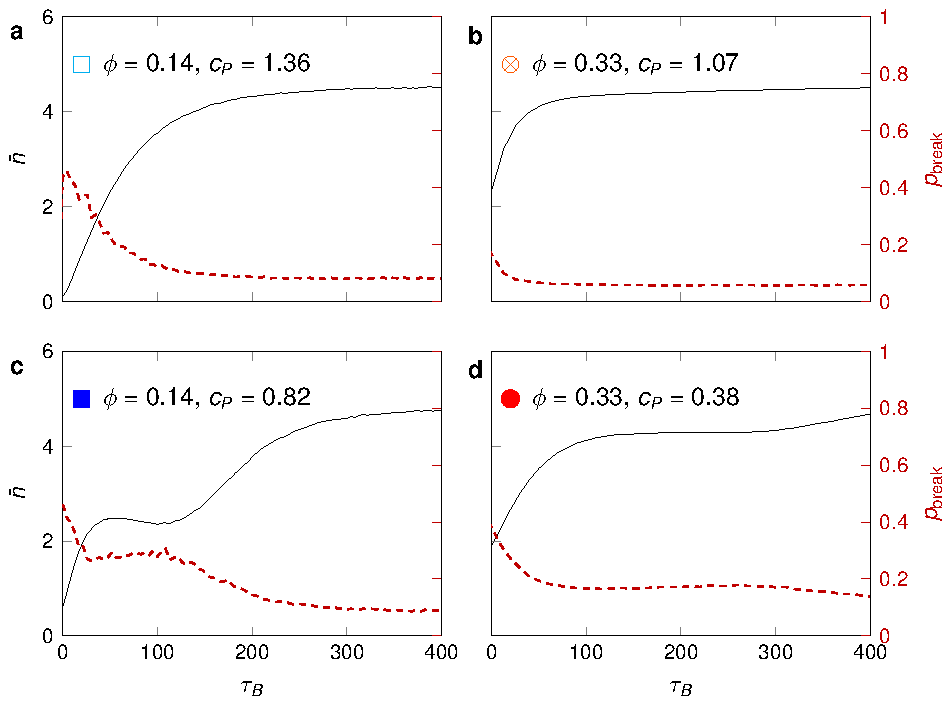
\includegraphics[width=10cm]{bond_breaking.pdf}
 \caption{{\bf Stress driven aging.} Time evolution of the average coordination of colloidal particles $\bar{n}$ (black continuous line) and the bond-breaking probability $p_\text{break}$ (red dashed line) for four gel samples. Symbols relate each sample to its position on the phase diagram \textcolor{blue}{in} Fig.~\ref{fig:network_formation}. $p_\text{break}$ is measured as the probability of bond breaking in a time interval of $\Delta t=10$ s. For high polymer concentration, panels {\bf a} and {\bf b}, $p_\text{break}$ decreases monotonically until it reaches a stationary state at long times, with $\bar{n}$ saturating at an average of less than $5$ neighbours. For low polymer concentration, panels {\bf c} and {\bf d}, $p_\text{break}$ follows a similar decay at intermediate times, with $\bar{n}$ less than $5$ neighbours, but which is then followed by a second decay to new configuration, where $\bar{n}$ becomes greater than $5$ neighbours.}
 \label{fig:bond_breaking}
\end{figure}

\textcolor{blue}
{
\textcolor{red}{From initial to intermediate times, before percolation is complete}, hydrodynamic interactions play a fundamental role~\cite{tanaka2000,tanaka2007spontaneous,furukawa2010key}.
Without hydrodynamic interactions, as often assumed in simulations, particles have the tendency to aggregate in compact structures and subsequently form thick network structures. This also limits to relatively high volume fractions the possibility to form arrested gel states. 
With hydrodynamic interactions, particles first form a transient gel even at very low volume fractions, and the number of nearest neighbours increases only later to minimize the energy of the structure. Thus, hydrodynamic interactions lead to the formation of gels that are very far from equilibrium and under a strong thermodynamic driving force towards more stable compact structures. The resulting transition from open to more compact networks occurs through the breaking of the bonds that have accumulated more stress. This process has been called stress-driven ageing~\cite{tanaka2007spontaneous}, and is characteristic of viscoelastic phase separation \cite{tanaka2000viscoelastic}. Whether the network undergoes such restructuring or not depends on the strength of the bonds, i.e. the polymer concentration.
In Fig.~\ref{fig:bond_breaking} we plot the bond breaking probability, $p_\text{bond}$, and the average coordination, $\bar{n}$, as a function of the time elapsed since salt injection ($t=0$).
At high polymer concentrations (panels \textbf{a}, \textbf{b}), $p_\text{break}$ decreases monotonically, until a stationary state is reached where $\bar{n}<5$.
At low polymer concentrations (panels \textbf{c}, \textbf{d}), the initial decay of $p_\text{break}$ to a network with $\bar{n}<5$ is followed by a secondary decay to a more compact network with $\bar{n}>6$. This means that mechanical stress built up in the first transient network can relax to a more compact network only when bonds are weak enough, i.e. at low polymer concentrations.
}

\textcolor{blue}{
It is worth noting that the two-step beheviour of $p_\text{break}$ and $\bar{n}$ is not due to crystallization, as this only starts after the network reorganization. For example, the fraction of crystalline particles for all frames in Fig.~\ref{fig:bond_breaking}d is always below $0.3\%$.
The increase in number of bonds after network reorganization is a necessary condition for crystallization, as we will show in the following, while in its absence the network forms low-density arrested states (gels).
 }
%In Fig.~\ref{fig:stress}a, we plot the fraction of liquid and gas particles as a function of time during phase separation at the state points of $\phi\approx 0.13$. We observe that at high polymer concentration ($c_p=1.36$, dashed lines) both the liquid and gas branch change monotonically with time as the phase separation proceeds. At low polymer concentration ($c_p=0.82$, continuous lines), on the other hand, we find a non-monotonic evolution of both the liquid and gas branches, which is signalling a structural reorganization of the network. To prove that this is indeed a stress-driven ageing process, in Fig.~\ref{fig:stress}b we plot the average number of bond-breaking events for the low-polymer concentration state point. The figure clearly shows that the network restructuring follows a peak in the number of bond-breaking events. We have thus found direct evidence of the stress-driven ageing process in colloidal gels that is a direct consequence of the formation of a thin network with the help of 
hydrodynamic interactions in the first stages of the aggregation process.
 
%In Fig.~\ref{fig:stress}c we plot the time evolution of the structure factor, $S(q)$, for the state point undergoing network reorganization $\phi\approx 0.13$ and $c_p=0.82$. The time of network reorganization as found in Fig.~\ref{fig:stress}a and b corresponds to a steep increase of the low wavenumber scattering from the network, that signals the coarsening of the network structure. 

%The same conclusions also hold for the state point at $\phi\approx 0.30$. We observe network restructuring only for the state point at lower polymer concentration, $c_p=0.38$. Interestingly, this is also the only state point that undergoes crystallization, meaning that the coarsening of the network of the dense liquid phase and the resulting formation of a wider liquid branch is a necessary condition for crystallization. 

%%%
%\subsection{Late times: dynamic-arrest vs crystallization}

\begin{figure*}
 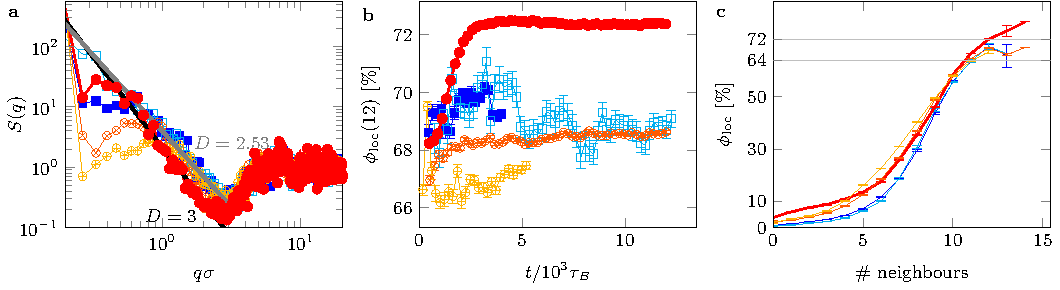
\includegraphics[width=16cm]{late_structure.pdf}
 \caption{\textcolor{blue}{{\bf Structural evolution at late times.}} 
{\bf a,} Structure factors for the late stages of the gelation process. The gray and black lines represent respectively random gelation and compact fractal dimensions.
{\bf b,} Late stage of the evolution of the local volume fraction \textcolor{blue}{$\phi_{\rm loc}$(12)} around colloidal particles having 12 nearest neighbours.
{\bf c,} Local volume fraction \textcolor{blue}{$\phi_{\rm loc}$} around a colloidal particle, as a function of the number of nearest neighbours of the particle for the state points in the very late stage. 
The two horizontal straight lines indicate the characteristic volume fractions in attractive systems, crystal ($\sim 0.72$) and glass ($\sim 0.64$).
Samples are shown with the same colour code as in Fig.~\ref{fig:network_formation}. In particular red circles correspond to the crystallizing sample at $\phi=0.33$ and $c_p=0.38\,$mg/g.
 }
 \label{fig:late_structure}
\end{figure*}

\textcolor{blue}{The samples share the same early stages of the phase separation process, but show significantly different behaviours in the later stages.}
To examine this in more detail, we plot in Fig.~\ref{fig:late_structure}a the structure factor for the final stages of the gelation process for all state points.
%Calculation of the structure factor is done with the Hanning window function, to minimize boundary effects.
At low wavenumber $q$, the structure factor displays fractal scaling compatible with the Guinier law, $S(q)\sim q^{-D}$.
But a difference in the fractal (or effective) dimension $D$ between the $\phi\approx 0.33$ and $c_p=0.38$ mg/g state point and other state points starts to become visible. In fact, while states
with high polymer concentration retain the exponent $D=2.5(3)$, 
which is the random gel universality class exponent, as we also observed in the early stages of the gelation process (see inset of Fig.~\ref{fig:network_formation}),
the state point with low polymer concentration ($\phi\approx 0.33$ and $c_p=0.38$ mg/g) displays the biggest deviation from that exponent. In the figure we also
plot the exponent $D=3$, which corresponds to volume growth, which we will show in the following analysis to be the correct exponent for this state. 
The difference is due to the onset of crystallization in the low-polymer concentration sample. This is already evident in the high $q$ behaviour of
the structure factors (Fig.~\ref{fig:late_structure}a), where the diffraction planes appear as sharper peaks for $\phi\approx 0.33$ and $c_p=0.38$ mg/g.

To gain additional insight, in Fig.~\ref{fig:late_structure}b we plot the late stage (after all samples already underwent gas-liquid phase separation) time evolution of the local volume fraction $\phi_\mathrm{loc}$ of closed packed particles (having 12 neighbours). The volume fraction is obtained by computing the Voronoi diagram of each configuration, which uniquely assigns a volume to each colloidal particle. Only the state point at $\phi\approx 0.33$ and $c_p = 0.38\,$mg/g shows an increase, up to an asymptotic value that we identify with the composition of the stable crystal phase $\approx 0.72$. We plot the asymptotic average volume fraction as a function of the number of neighbours in Fig.~\ref{fig:late_structure}c. Approaching close packing (12 neighbours), we clearly see two families of curves. The state point at $\phi\approx 0.33$ and $c_p=0.38\,$mg/g reaches close packing at the volume fraction $\approx 0.72$. By contrast, all other state points reach close packing at a markedly 
lower volume fraction, which is indeed close to the volume fraction of the attractive glass state~\cite{pham2002multiple}.  \textcolor{blue}{These structural analysis provide some evidence that the state point $\phi\approx 0.33$ and $c_p=0.38\,$mg/g could be following a different arrest mechanism, in which phase separation is arrested by crystallization and not by glassiness. In the reminder of this manuscript we investigate this state more closely, to confirm these early results.}


%To gain additional insight, in Fig.~\ref{fig:late_structure}c we plot the average local volume fraction as a function of the number of neighbours.
%\textcolor{blue}{The volume fraction is obtained by computing the Voronoi diagram of each configuration, which uniquely assigns a volume to each colloidal particle.}
%For all state points, we can see that the average volume fraction of a colloidal
%particle increases with its number of neighbours. Approaching close packing (12 neighbours), we clearly see two families of curves. \textcolor{blue}{The state point at $\phi\approx 0.33$ and $c_p=0.38\,$mg/g reaches close packing at the
%volume fraction $\approx 0.72$ of the stable crystal phase. By contrast all other state points, reach close packing at a lower volume fraction, which is indeed close to the volume fraction of the attractive glass state~\cite{pham2002multiple}. 
%%~\cite{ilett1995phase}
%% 
%The time evolution  of the local volume fraction of particles having 12 neighbours is also informative, see Supplementary Figure~\ref{S-fig:local_phi12}. After all samples underwent gas-liquid phase separation, only the state point at $\phi\approx 0.33$ and $c_p = 0.38\,$mg/g state shows an increase, up to an asymptotic value markedly higher than all other samples. 
%(\textbf{the absolute values of these volume fraction are not totally convincing, probably because of a not optimal estimate of the size of the colloids. We should run the code of Mathieau with size detection}). 
%This result clearly indicates that this state point} follows a different arrest mechanism, in which phase separation is arrested by crystallization and not by glassiness. %Although our estimation of the absolute volume fraction may involves systematic errors of a few \%, the trend should be robust~\cite{Poon2012}.


% 
%  REINTREGRARE
% while the crystallizing state point shows a scaling compatible with $D=3$, which
% signals compact crystalline nuclei. At high $q$, the first signals from diffraction planes are also evident in the $\phi\approx 0.30$ and $c_p=0.38$ state
% point. This suggests that the space filling network is composed of crystalline aggregates, differently from the fractal branches which characterize the
% spinodal liquid. Also this suggests that the growth mechanism of the crystal is not simply due to filling of the spinodal liquid network, as was
% instead observed in Ref.~\cite{soga1999metastable,fortini2008crystallization,perez2011pathways} for brownian dynamics simulations.

\begin{figure}
 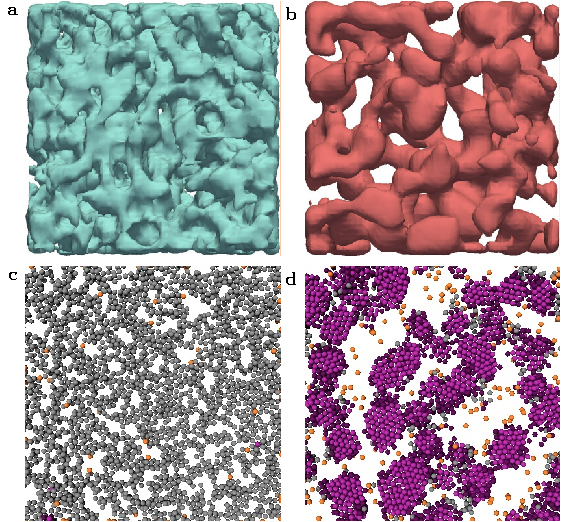
\includegraphics[width=10cm]{network}
 % crystal_size.eps: 0x0 pixel, 300dpi, 0.00x0.00 cm, bb=(atend)
\caption{{\bf Percolated network structures.} 
{\bf a, b:} the network is represented in a coarse-grained fashion (see Methods).
{\bf c, d:} slabs of 4.5 $\mu$m thickness and 41 $\mu$m width. Particles are drawn to scale and coloured according to their phase. Purple: crystal; dark purple: crystal surface; gray: liquid; orange: gas. 
{\bf a, c:} a gel obtained from the state point $\phi\approx 0.33$ and $c_p=1.07$ mg/g at $t=400$ min after sample preparation. 
{\bf b, d:} a crystal-gel at the same $\phi$ but at lower polymer concentration, $c_p=0.38$ mg/g at $t=468$ min after sample preparation. 
On the top row we can clearly see not only the percolated nature of both networks, but also the difference in the smoothness of the network surface between amorphous and crystal gels. 
We note that very few liquid particles remain in \textbf{d} and the network is almost crystalline. 
} 
\label{fig:network}
\end{figure}

A direct analysis of the colloidal positions at late times confirms that indeed the new structure obtained at $\phi\approx 0.33$ and $c_p=0.38$ mg/g has different morphological properties than usual colloidal gels.
We directly compare the two structures in Fig.~\ref{fig:network}a and b, where Gaussian filtering is used to depict the network structure as a continuous field (see Methods).
Panel~a presents the results for high polymer concentration gel, $c_p=1.07$ mg/g \textcolor{blue}{that never undergoes stress-driven ageing}; panel~b presents the results for the low polymer concentration sample, $c_p=0.38$ mg/g.
The comparison shows that the new arrest mechanism produces a \textcolor{blue}{beaded} network structure with bigger pores, smoother surfaces \textcolor{blue}{(consistently with $D=3$)}, and thicker strands (panel b) compared 
to the colloidal gel sample (panel a). The bottom row shows the individual particle positions for slabs with a thickness of 5 particle diameters. 
From the figure it is immediately clear that the network strands at low polymer concentration are crystalline. The new arrest mechanism thus
involve the formation of a crystal-gel network. In order to explain the morphological differences between colloidal gels \textcolor{blue}{(networks made of thin strands)} and crystal-gels \textcolor{blue}{(networks made of thick crystal beads)},
we now consider the kinetics of formation in our samples. 

\begin{figure}
 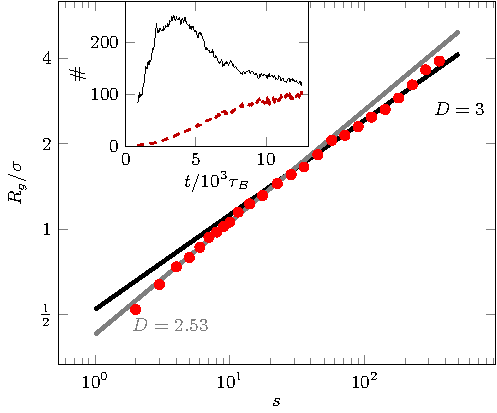
\includegraphics[width=8cm]{characterisation}
 % crystal_size.eps: 0x0 pixel, 300dpi, 0.00x0.00 cm, bb=(atend)
\caption{{\bf Characterization of the crystal-gel.} 
Radius of gyration of crystalline nuclei at the late stages of gelation for the state point $\phi\approx 0.33$ and $c_p=0.38$ mg/g.
The gray and black straight lines have a slope of $1/2.53$ and $1/3$ respectively. 
\textbf{(Inset)} Time evolution of the average size of the crystals \textcolor{blue}{(red dashed line)} and the number of crystals 
\textcolor{blue}{(black line)} for the same state point.
} 
 \label{fig:crystals}
\end{figure}


Supplementary Movie 2 shows the late stage (after the initial spinodal decomposition) evolution of a 2D confocal slice. Even on this raw data the growth of crystalline regions is obvious. More quantitatively, we adopt bond orientational analysis to detect which particles are in crystalline environments~\cite{russo2013interplay} 
(see Supplementary Information on the detail). 
With this analysis we reveal that crystallization events indeed start occurring for the state point $\phi\approx 0.33$ and $c_p=0.38$ mg/g, which has the lowest
polymer concentration of all state points. This is shown in the inset of Fig.~\ref{fig:crystals}, where the \textcolor{blue}{red dashed} line indicates the average size of the crystallites, 
while the \textcolor{blue}{black} line indicates the average number of crystallites as a function of time. The number of crystallites first rapidly increases as nucleation events
start occurring inside the liquid network, but eventually starts decreasing as the different crystallites grow and merge with each other.  Supplementary Movie 3 shows a three-dimensional (3D) reconstruction  of the whole phase ordering sequence that emphasizes crystalline particles. Although crystal clusters are isolated in this movie, they are bridged by the dense colloidal liquid phase and involved in the percolated gel network, as can be seen in Fig. \ref{fig:network}b and d. 
We can see that crystal clusters grow by condensation from the colloidal gas phase. 
%The average size of the crystals shows an interesting linear growth regime for $100<t<600$. This linear growth regime goes past the time
%of coalescence of nuclei, so a first speculation is that it could be due to the compensation of the following two effects:
%\begin{itemize}
% \item diffusive growth of the nuclei, which scales like $t^{1/2}$
% \item coalescence growth, which should scale faster than $t$, maybe $t^2?$
%\end{itemize}
All other state points show only negligible signs of crystallization. In particular, for state points with $\phi\approx 0.33$, increasing
polymer concentration drastically reduces the amount of crystals. This is in agreement with the
idea of enhanced crystallization rates near metastable critical points~\cite{ten1997enhancement,olmsted1998spinodal} and the
results of Refs.~\cite{soga1999metastable,fortini2008crystallization,perez2011pathways},
which speculated two different arrest mechanisms: crystallization at low polymer concentration, and dynamic arrest at high polymer concentrations.

%\subsection{Crystal-growth routes}

\begin{figure*}
 \centering
 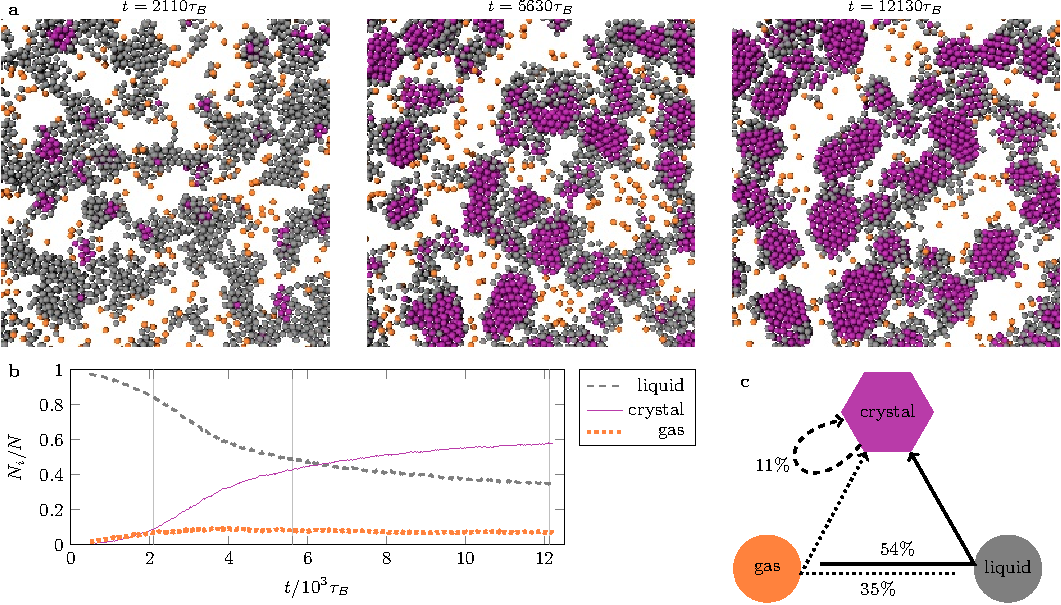
\includegraphics[width=16cm]{transitions}
 % snapshots.eps: 0x0 pixel, 300dpi, 0.00x0.00 cm, bb=0 -1 2256 735
 \caption{{\bf Crystal gel formation.}  
{\bf a,} Reconstructions from confocal coordinates at $\phi\approx 0.33$ and $c_p=0.38$ mg/g. The depth of view is 9.0 $\mu$m, while the lateral dimension is 41 $\mu$m. Particles are drawn to scale and coloured according to their phase. Purple: crystal; dark purple: crystal surface; gray: liquid; orange: gas.
{\bf b,} Fraction of particles for each phase. Gray vertical lines indicate the times shown in panel a. 
{\bf c,} Sketch of the three routes by which a particle can end up in a crystal state. 
Probabilities are computed from the history of each single trajectory. 
A trajectory without liquid evaporation or crystal sublimation is counted as direct crystallization (continuous arrow, 54\%). 
If a liquid particle evaporates and then de-sublimates it counts in the Bergeron process (dotted arrow, 35\%). 
If sublimation is followed by de-sublimation it is Ostwald ripening (dashed arrow, 11\%). 
Most trajectories proceed via the surface state.}
\label{fig:transitions}
\end{figure*}

While nucleation always occurs inside the liquid branches of the phase-separating network, crystal growth can proceed through different growth \textcolor{blue}{routes}.
In the following we will show that the growth mechanism of the crystal is not only due to filling of the spinodal liquid network, as was observed in Refs.~\cite{soga1999metastable,fortini2008crystallization,perez2011pathways} for Brownian Dynamics simulations, but also involves the Bergeron process and Ostwald ripening. 
In Fig.~\ref{fig:crystals} we show the gyration radius of individual crystalline nuclei for the state point 
$\phi\approx 0.33$ and $c_p=0.38$ mg/g. The results show that the crystal growth follows two different scaling laws: at small crystalline sizes it scales with 
the fractal (or effective) dimension close to random percolation ($D=2.53$), while at large sizes it scales as $D=3$, as in compact crystal growth. This demonstrates that, while 
small crystalline nuclei are nucleated inside the phase-separated liquid branches, once they reach the transverse size of the liquid branch, the growth 
follows a volume growth with the formation of isotropic crystal droplets. The same scaling law was suggested in the analysis of the
structure factors, Fig.~\ref{fig:late_structure}a, but here it is shown directly by the analysis of the gyration radius. 

Next we analyse in detail the crystallization trajectory, distinguishing between the different processes responsible for the
crystallization of the phase separated network.
%Supplementary Movies 2 and 3D show the time-lapse videos of 2D confocal microscopy observation and 3D computer reconstruction, respectively, for the crystallizing sample at $\phi\approx 0.33$ and $c_p=0.38$ mg/g,
%where the process of crystal growth by direct attachment of gas particles can be observed directly. 
From the trajectory, we extract slabs of 10 particle diameter thickness for configurations at different times, shown in Fig.~\ref{fig:transitions}a. 
Particles are coloured according to their phases (gas, liquid, and crystal). For the classification criteria, see Supplementary Information. The figure shows the first nucleation 
events inside the liquid network (left panel). At the same time liquid regions that have not crystallized start evaporating, and the gas phase contributes to the growth of crystal nuclei (middle panel). Finally the different nuclei coalesce (right panel). 
Note that the topology of the crystal network found at late times, i.e. $t=5577\,\tau_{\rm B}$ (middle panel) and $t=12098\,\tau_{\rm B}$ (right panel) in Fig.~\ref{fig:transitions}a, differs significantly from that of the liquid network at early stages, i.e. $t=2055\,\tau_{\rm B}$ (left panel) in Fig.~\ref{fig:transitions}a. This suggests that the crystal network does not form only by direct freezing of the liquid, but also by other mechanisms which involve the evaporation of the liquid (Bergeron process) and the sublimation of small crystals (Ostwald ripening). In the following we will investigate these different crystallization mechanisms in depth.
 


In Fig.~\ref{fig:transitions}b, we show  the fraction of particles in each different phase for the crystallization trajectory at
$\phi\approx 0.33$ and $c_p=0.38$ mg/g, after the liquid-gas phase separation has occurred.
The process of crystallization is characterized 
by a steep decrease in liquid particles, as they transform into small crystalline nuclei inside the liquid domains. This decrease
is then accompanied by an increase in the fraction of gas particles: as the first crystals start to reach the gas phase, liquid particles evaporate 
to the gas phase due to the higher vapour pressure of the liquid phase compared to the crystalline phase. 
After the onset of a steady-state gas population, there are three growth routes for the crystal. 
Direct crystallization is the process by which crystals grow by incorporating nearby liquid particles. 
In the Bergeron process, liquid droplets first evaporate and the resulting gas phase contributes to the growth of crystalline regions. Ostwald ripening is instead the process by which small crystallites sublimate, and colloidal particles are transferred to larger nuclei.
\textcolor{blue}{Since we have access to individual particle trajectories, we can directly assess the relative importance of these three growth channels.}
For every time frame, we assign each particle a state between gas, liquid and crystal. In order to minimize short-term fluctuations, the state of each colloidal particle is time averaged for $50\,\tau_{\rm B}$. We then measure the fraction of trajectories with different transition histories.
The different crystallization routes are depicted in the diagram of Fig.~\ref{fig:transitions}c.
Direct crystallization accounts for 54\% of particles trajectories in which gas or liquid particles transition to the crystal state without liquid evaporation or crystal de-sublimation. 
The Bergeron process accounts for 35\% of particle trajectories in which liquid particles transition to the gas state before crystallizing. 
Ostwald ripening accounts for 11\% of particle trajectories in which crystal particles transition to the gas state before returning to the crystal state. \textcolor{blue}{Here we note that the Bergeron and Ostwald ripening processes both take place only when the crystallites are 
surrounded by the gas phase due to the non-existence of a liquid-crystal coexistence. Such a gas-crystal coexistence was speculated  by Poon and his coworkers on the basis of free-energy argument \cite{poon1999cpm,renth2001phase}.} 
 


In Supplementary Information we confirm these results with a detailed analysis of transition probabilities, including a state for surface particles that are in contact 
to crystalline particles, see Supplementary Figure~\ref{S-fig:probabilities}.
While the direct freezing of the fluid represents the major contribution to the nuclei growth, the kinetic path via the gas phase (gas$\rightarrow$crystal), also plays a crucial role,
especially in determining the morphology of the porous crystal, as we discussed above. In this context the Bergeron process~\cite{glickman2000glossary,morrison2012resilience}
plays a considerably more important role than Ostwald ripening \textcolor{blue}{and is responsible for the beaded network morphology}.

% 
% Here we mention the simulations closer to our experimental results~\cite{fortini2008crystallization}.
% It was shown there that close to the metastable liquid-gas critical point, the gelation process is arrested by
% crystallization, while at higher polymer concentration by slow dynamics. This is roughly what we observe in
% our experiments, but there is a crucial difference. In the simulation results~\cite{fortini2008crystallization} the kinetic
% pathway at volume fraction $\phi\approx 0.30$ consists of the following three steps: 
% spinodal decomposition; nucleation of crystalline nuclei within the fluid branches;
% growth of crystalline clusters until the whole spinodal structure is crystalline.
% As shown above, the last step appears to be markedly different in our experiments.
% More precisely, at $\phi\approx 0.30$ and polymer concentration $c_p=0.38$ we also observe the first two steps, 
% but the growth process is entirely different. Instead of growing inside
% the spinodal aggregate, the small nuclei grow by adding colloids directly from the gas phase. 

%\subsection{Discussion and conclusions}
The first stages of gelation always involve spinodal decomposition with the formation
of liquid network by viscoelastic gas-liquid phase separation. 
% Due to hydrodynamic interaction, the network is locally stretched, and the accumulation of mechanical stress on some bonds causes some
% of them to break and the network to reorganize in a more compact and larger structure. This occurs only at low polymer concentration,
% while at high polymer concentrations the bonds are too strong to break. This will eventually dictate which arrest mechanism
% is available to the system.
Depending on the polymer concentration, there are two possible arrest mechanisms. 
\textcolor{blue}{(a) Crystallization: small crystalline nuclei appear inside the liquid network, reach the surface 
 of the liquid branches, and then grow by addition of particles from the gas phase. The final structure is a network of crystal droplets,
 as confirmed by the fractal dimension of the branches, the volume fraction of the particles within the branches, and bond orientational analysis. 
(b) Dynamic arrest: particle arrest when the dynamics inside the liquid branch becomes slow, which should happen at the intersection of the  glass line with the liquid side of the coexistence curve.}

\textcolor{blue}{In our system, mechanism (a) is operative around $\phi\approx 0.33$ and $c_p=0.38$ mg/g. 
The physical conditions required for the crystal-gel formation revealed in our study indicates that the extent of the $\phi$-$c_p$ region where mechanism (a) is operative can be widened by changing the location of the critical point, which in our system is controlled by the size of the non-adsorbing polymer: moving the critical point to lower polymer concentrations opens the window where bonds can rearrange before the intervening glass transition. So we argue that the region of formation of crystal-gel porous structures is not only easily accessible, but also controllable.}


The Bergeron process is also the primary mechanism for the formation of rain drops in clouds~\cite{glickman2000glossary,morrison2012resilience}.
In clouds there is a mixture of ice crystals and supercooled water. The vapour phase is in coexistence with the liquid phase, but is supersaturated
with respect to the ice crystals. This causes the water droplets to evaporate and de-sublimate directly on the ice crystals. Our system can then
be regarded as a colloidal analogue for this important process, which, for the first time, we can observe at the single-particle level.  

The process of formation of ``crystal gels'' may be generic to many other 
systems. The requirements are (i) the presence of gas-liquid phase separation below the melting point of a crystal, (ii) 
weak or little frustration against crystallization (in our case, the use of monodisperse colloids), 
(iii) dynamical slowing down in a supercooled liquid state, which is necessary to induce viscoelastic phase separation leading to the formation 
of a network structure of the minority liquid phase, and (iv) the degree of supercooling is low enough
\textcolor{blue}{to allow bond-breaking events that avoid the vitrification of the liquid phase.}
Many monoatomic and single-component molecular systems can satisfy all these conditions in a certain range of the temperature and pressure. 
This can be seen, for example, by looking at the phase diagram of a Lennard-Jones liquid \cite{lodge1997brownian}, which represents many molecular systems 
without specific directional interactions. For monoatomic systems such as noble metals, condition (iii) may not be satisfied easily. 
To access glassy slow dynamics in a liquid phase, we may need a deep quench at a high pressure. However, we note that even without strong dynamic asymmetry 
due to glassiness, bicontinuous phase separation can take place between 35-85 volume \% of the liquid phase in ordinary gas/liquid phase separation \cite{Onuki2002}; 
and, thus, porous crystalline structures can be formed, although a thin network structure may be difficult to be formed.

Usually, monoatomic systems are very poor glass-formers and thus have not been expected to form gels. 
However, our mechanism provides a novel kinetic pathway to spontaneously form network or porous structures made of crystals.  The fact that crystals outgrow from the liquid network means that well-ordered crystal planes appear on the surface of the porous structure (see Fig. 2b), which is crucial for catalytic and sensing applications. So we believe that crystal gels are an important class of heterogeneous non-ergodic states in nature 
and industrial applications, although they have not attracted much attention so far.  
For example, nano-porous crystals of noble metals such as Au have special functions associated with ultra-high interfacial area and connectivity of pores, which are relevant to catalytic, optical, sensing, super-capacitor, and filtration applications 
\cite{ding2004nanoporous, ding2009nanoporous, wittstock2010nanoporous,fujita2012atomic}. Usually such nano-porous materials are formed via at least two steps: for example, phase separation and dealloying of a mixture
\cite{erlebacher2001evolution}. Unlike such a method, our novel mechanism allows us to spontaneously form sponge-like nano-porous crystals \emph{in a single step}, 
which may have an impact on many applications. 
We note that laser ablation of metals is a promising method for this purpose \cite{povarnitsyn2013mechanisms}.
We also speculate that our scenario could play a role in the formation of crystal networks observed in dynamically asymmetric mixtures, 
which includes magma \cite{philpotts1998role}, biominerals \cite{rousseau2005multiscale}, and foods \cite{deman1987fat}. 

\section*{METHODS}

\subsection*{Experiments}

We use \textsc{pmma} (poly(methyl methacrylate)) colloids sterically stabilized with methacryloxypropyl terminated \textsc{pdms}(poly(dimethyl siloxane)) and fluorescently labelled with rhodamine isothiocyanate chemically bonded to the \textsc{pmma}.
The diffusion constant in dilute conditions without polymer allows us to estimate the colloid diameter to $2.3\pm 0.05\, \mu$m. The Brownian time is $\tau_{\rm B} \approx 2.3\,$s. 
We assess that the size distribution of our particle is Gaussian with a polydispersity below 5\% via direct confocal measurements~\cite{Leocmach2013}.
This small polydispersity allows crystallization.
We disperse the particles in refractive index and density matching mixture of cis-decalin (Tokyo Kasei) and bromocyclohexane (Sigma-Aldrich). 
The precision of density matching is $\sim 10^{-4}$ mg/ml, for which the gravity effect on our gelation processes is negligible up to 12 hours.

To induce short-ranged depletion attraction, we use polystyrene (TOSOH) as non-adsorbing polymer of molecular weight 3.8 MDa.
Experiments are conducted at 27 $^\circ$C, some 80 $^\circ$C above the theta temperature in this solvents mixture~\cite{Royall2007}. A Flory scaling of the measurements of~\cite{lu2008gelation} yields a radius of gyration $R_g=76\pm5$ nm.

Matching phase boundaries often leads to better determination of volume fractions than colloid diameter measurements~\cite{Poon2012}. We obtain the best match between theoretical phase diagram and experimental data for $\sigma=2.21\,\mu$m and $R_g=80$ nm (see Supplementary Method). Therefore the polymer-colloid size ratio is $q_R=2R_g/\sigma=0.072$ and the overlap mass fraction of polymer $2.25$~mg/g.

In the absence of salt, the Debye length is expected to reach a few micrometers and the (weakly) charged colloids experience a long range electrostatic repulsion. We confirm that colloids never come close enough to feel the short-ranged attraction. Screening by tetrabutylammonium bromide (Fluka) at saturated concentration brings down the Debye length to about 100~nm practically discarding the repulsion. 
Thus, salt introduction can screen the Coulomb repulsion and make the polymer-induced depletion attraction effective, initiating phase separation. 

\textcolor{blue}{To avoid solvent flow upon salt addition, our sample cell has two layer compartments separated by a membrane filter of pore size of 0.1 $\mu$m, permeable only to polymers and the salt ions. The top layer is 200 $\mu$m thick and contains the sample: a mixture of colloids, polymer, and solvent without salt. The bottom layer is a salt-reservoir with a half-opened structure, which allows us to exchange or insert a reservoir solution. The volume ratio of the first and second compartments is approximately 1:100.}

In our experiments, the reservoir solution is initially a polymer solution without salt and electrostatic repulsion by the unscreened surface charges inhibited colloidal aggregation. Under microscopy observation, we quickly exchange the reservoir solution to a polymer solution with salt at saturated concentration (4 mM) and seal the half-opened reservoir with cover glass to avoid evaporation of solvent. Salt diffuse into the first layer within a few minutes, typically 2 minutes, screen the surface charges, and initiat colloidal aggregation. This allows us to observe the process without suffering from harmful turbulent flow.

The data are collected on an upright Leica SP5 confocal microscope, using 532 nm laser excitation. The scanning volume is 98 $\times$ 98 $\times$ 53 $\mu$m$^3$, which contains $\sim 10^4$ colloid particles. Our spatial resolution is 192 nm / pixel. To be able to follow individual trajectories, we perform a 3D scan every 10~s ($\approx 4\tau_{\rm B}$) at early time and every 30 s later.


The crystal-gel state is reproduced in a sealed cell with all the components of the suspension pre-mixed. The colloid volume fraction is virtually identical at $\approx 0.33$ and polymer concentration is $0.40\,$mg/g. See Supplementary Figure~\ref{S-fig:capillary}.





%\paragraph*{State points studied}
%The experimental data is taken at two different volume fractions ($\phi=0.10$ and $\phi=0.25$) and for different values
%of the polymer concentration, $c_p=0.38,0.48,0.57,1.07$ for $\phi=0.25$ and $c_p=0.82,1.36$ for $\phi=0.10$.
%For each state points, scans at early times (every $10s$) and at the late stage (every $30s$) of the gelation process.
%
%We will consider two particles bonded if their centre-to-centre distance is within $12$ pixels. The radius of a colloidal
%particle is $5.365$ pixels.

\subsection*{Structural analysis}

\textcolor{blue}{Calculation of the structure factor is done with the Hanning window function, to minimize boundary effects. To account for imprecision in particle localisation close to contact, we consider two particles bonded if their centre-to-centre distance is within 2.4~$\mu$m, which is the range of the potential ($\sigma+2R_g$) plus our worse estimate of localisation inaccuracy (0.15~pixels)~\cite{Leocmach2013}.}

To detect percolation, two different methods have been employed. In the first one we detect percolation by looking at which frame the cluster size distribution has a more extended power-law decay. 
In the second technique, we simply measure the spatial extent of the largest cluster and consider it percolating when it is comparable to the size of the field of view of the microscope. 
Both methods lead to essentially identical percolation time for each state point.

\textcolor{blue}{Coarse-grained representation of the network is obtained by applying a Gaussian filter to the position of the particles (of width equal to the inter-particle distance) and plotting the surface which bounds the highest 20 \% values of the field.}


\bibliographystyle{naturemag2}
\bibliography{biblio}

\bigskip
\noindent
{\bf Acknowledgements} 
This study was partly supported by Grants-in-Aid for Scientific Research (S) (Grand No. 21224011) and Specially Promoted Research (Grand No. 25000002) from the Japan Society for the Promotion of Science (JSPS). 

\medskip
\noindent
{\bf Author Contributions} 
H.Ts. and J.R. contributed equally to this work. 
H.Ta. conceived and supervised the project, H.Ts. performed experiments, J.R. analysed the data, M.L. linked experiments and analysis, and all the authors discussed and wrote the manuscript. 

\medskip
\noindent
{\bf Additional information} 
%Reprints and permissions information is available at www.nature.com/reprints.
Correspondence and requests for materials should be addressed to H.T. 

\medskip
\noindent
{\bf Competing financial interests}
The authors declare no competing financial interests

\end{document}



